\begin{section}*{Assignment 1}
 \subsection{Algemeen}
Deze handleiding is opgesteld voor leerkrachten die wensen een klas te registreren binnen de Bebras Applicatie. Zoals u wellicht al weet is er naast het online registreren van een klas (via de webapplicatie) ook een mogelijkheid om klassen te registreren door met behulp van spreadsheets. \\
In deze handleiding leggen we stap voor stap uit hoe u klas(sen) succesvol kan registreren binnen de applicatie. Dit in de veronderstelling dat de lezer een basiskennis bezit over het gebruik van de webapplicatie zelf alsook het gebruik van excel of andere rekenblad-applicaties.
\subsection{Registratie}
Het registreren van een klas of meerdere klassen kan worden gerealiseerd door het gebruik van een spreadsheet of digitaal rekenblad. Dit is een verzameling van werkbladen die bestaan uit cellen die samen een tabel vormen. Het gebruik van dergelijke sheets laat het toe om efficient bewerkingen uit te voeren op de aanwezige data (bv. het opvragen van data).\\
Voor de eigenlijke registratie begint u eerst met het openen van uw favoriet rekenblad-programma (zoals Microsoft Office Excel of de opensource alternatieven LibreOffice Calc en OpenOffice Spreadsheet). In deze handleiding zullen we werken met OpenOffice Spreadsheet.\\
\textbf{Merk op dat de registratie analoog is voor elk rekenblad-programma!}\\
\subsubsection{Werkblad openen}
\begin{center}
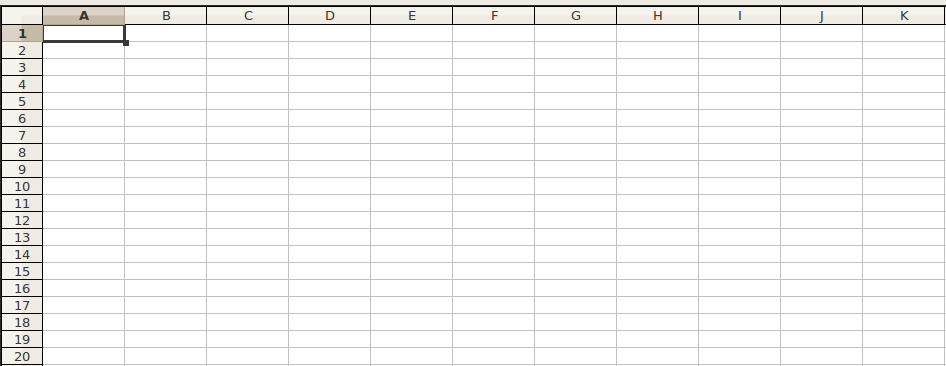
\includegraphics[height=4.5cm]{img/werkblad.png}
\end{center}
Bij het openen van uw applicatie ziet u een werkblad verschijnen waarin u duidelijk cellen kan opmerken. Elke kolom zal staan voor een ander informatieveldje. 
\subsubsection{Klas toevoegen}
Het systeem laat toe dat \textbf{meerdere klassen} kunnen worden geregistreerd binnen één werkblad. Om een klas te definieren beginnen we met in kolom A en een willekeurige rij (bv. 1) \texttt{\#CLASS\_B} in te vullen. Dit zal dienen om de applicatie duidelijk te maken dat een klassendefinitie begint (waarin leerlingen kunnen worden geregistreerd).\\
We gaan naar de volgende kolom waarin we de naam van de klas (naam die wordt gebruikt binnen de school) invullen (bv. \texttt{UGent}). Vervolgens zullen we in kolom C het level van de klas invullen (1-4) (bv. 1 : leeftijd 10-12). Tenslotte vullen we in kolom D de tijdsperiode in van de klas (bv. 2012-2013).\\
De volgende rijen zullen worden gebruikt voor het registreren van leerlingen. Indien alle leerlingen zijn geregistreerd plaatsen we in kolom A, op de volgende rij \texttt{\#CLASS\_E}. Hiermee maken we duidelijk dat een klassendefinitie stopt.\\
Het resultaat van deze stap wordt extra duidelijk gemaakt in de onderstaande afbeelding. 
\begin{center}
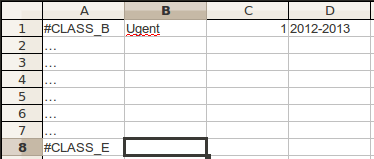
\includegraphics[height=3cm]{img/klas.png}
\end{center}
\subsubsection{Leerling toevoegen}
Binnen een klassendefinitie zal elke rij staan voor een welbepaalde leerling.\\
De volgende kolommen zullen worden gebruikt:
\begin{enumerate}
\item \textbf{A : } Achternaam (bv. Mortier)
\item \textbf{B : } Voornaam (bv. Thomas)
\item \textbf{C : } Geslacht(M$\vert$V) (bv. M)
\item \textbf{D : } Emailadres (bv. ThomasF.Mortier@UGent.be)
\item \textbf{E : } Eerste registratie(jaar) (bv. 2012-2013)
\item \textbf{F : } Geboortedatum(YYYY/MM) (bv. 1992/06)
\item \textbf{G : } Taal(FR$\vert$NL$\vert$EN) (bv. NL)
\end{enumerate}
Als voorbeeld heeft men de onderstaande afbeelding.
\begin{center}
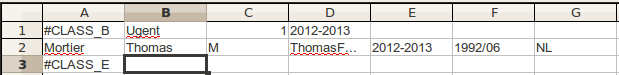
\includegraphics[height=1.39cm]{img/leerling.png}
\end{center}
Uit de bovenstaande afbeelding kunnen we dus de registratie afleiden van een klas (genaamd Ugent) met een graad 1 die geregistreerd is voor het jaar 2012-2013. Deze klas bevat slechts 1 leerling.
\subsubsection{Uploaden}
Na registratie slaat u uw werkblad op als een \textbf{XSLX} bestand. Hierna kan u dit bestand via de web applicatie openen waarna het bestand automatisch wordt verwerkt. Uw klas is tenslotte aangemaakt.
\end{section}
